\chapter{Introduction}
\epigraph{They're trying to understand what space is. That's tough for them.
They break distances down into concentrations of chemicals. For them, space is a
range of taste intensities.}{Greg Bear, Blood Music}
%
Countless manhours have been spent improving the design and manufacturing
process of the digital computer, creating more and more complex architectures
capable of operating at ever greater speeds.
%
The brain is not subject to this top down design philosophy, yet through a
process of self organization neurons are capable of forming highly complex
networks capable of solving complex tasks, with far greater energy efficiency,
robustness and parallellism than any designed processor.
%
Inspired by work done in the field of material computing systems such as the
mecobo platform of nascence [citation needed], a similar system has implemented
using living neural networks grown from human stem cells.
Neurons are grown \emph{in vitro} \footnote{From latin, literally ``in glass'',
as opposed to in the body.} on \emph{Micro Electrode Arrays} \ref{neuroIntro}:A,
C (MEA) are interfaced with a digital computer via voltage spike measurements
\ref{neuroIntro}:B, forming a hybrid neuro-digital system.
%
This system utilizes the theoretical framework of \emph{Reservoir Computing} to
help translate between the digital and biological parts of the system, allowing
it to solve simple tasks as a proof of concept.
%
The ultimate goal of the cyborg is to further our understanding of the
underlying principles that governing how nature computes.
\begin{figure}[h!]
  \centering
  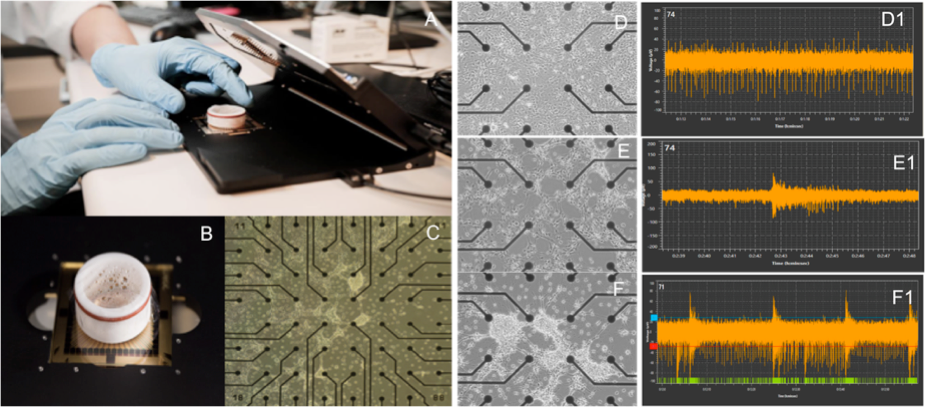
\includegraphics[width=1\textwidth]{fig/MEA_overview.png}
  \caption{From socrates webpage}
  \label{neuroIntro}
\end{figure}
\section{Complexity}
In the 50's and 60's there was much optimism in the burgeoning field of
artificial intelligence. In 1965 H. A. Simon claimed ``machines will be capable,
within twenty years, of doing any work a man can
do.''\cite{vardi_artificial_nodate} , while Marvin Minsky boldly claimed in 1967
that ``Within a generation ... the problem of creating 'artificial intelligence'
will substantially be solved.'' \cite{noauthor_marvin_nodate}.
Had they chosen to predict any other field, such as logistics, information
sharing or communications their statements would have been prophetic and
visionary, so why did artificial intelligence turn out so differently?
%
The researchers sought to make machines that could use logic similar to that of
high level human thinking.
%
Therefore, it followed that the machine had to be programmed with rules
governing logic in order to reach sound conclusions.
%
To represent the prior and deduced knowledge, the researchers designed
programming languages such as lisp that could accurately describe these
operations.
%
In order to actually execute these lisp programs hardware had to be created,
supporting the primitive operations such as addition, subtraction and loading
from memory.
%
Regardless of the underlying platform a lisp program did not change meaning, and
the binary adder in the heart of the processor never interacted with the
floating point adder. In short, each piece of the puzzle was self contained,
and the \emph{Complexity} of the systems behavior was similar to that of the sum
of its parts, which made it feasible to build large systems.
%
Nature, on the other hand, applies a completely different method.
Complex structures appear with no blueprint, arising from a process of
\emph{self-organization} driven by a set of growth rules. This self organizing
process is capable of producing incredibly complex, robust and diverse
structures whose functionality arises not from specialized components working in
isolation, but from the interaction of many components.
%
Applying the superposition principle to the processor makes sense, it allows us
to study each individual component in isolation before investigating how they
interact.
%
On the other hand, applying the superposition principle to nature leaves us
blind to the fact that the purpose of most components is to interact rather than
performing a specific function.\\
It seems the reason the researchers failed was their underestimation of the role
played by complexity, believing it was an incidental product of evolution rather
than a necessity.
TODO: En setning her som motiverer alt over. A la ``Derfor valgte va å lage en
cyborg i stedet for å dille med n-te ordens logikk i LISP.''

\section{Computation}
The invention of the digital computer will be remembered as one of, if not the
most significant technological advances of mankind.
%
With this neatly designed clockwork machine the concept of computation seemed
rather straight forward, where each executed machine instruction corresponded to
some unit of computation.
%
This idea of computation is very convenient, and it fails utterly when
applied to biological systems.
In a recent example of this from 2005 [Cite The Singularity Is Near: When Humans
Transcend Biology] Ray Kurzweil claimed that computers would be as powerful as a
mouse brain by 2020, a prospect that looks rather unlikely in 2018.
Other than in the head of computer scientists, neurons have no notion of
floating point operations or branching logic, and measuring the computational
capabilities of a brain in FLOPS is grossly underestimating what computing
\emph{can} be.
%
In spite of the digital computers shortcoming compared to the human brain, the
conventional digital approach to computing has been hugely successful in solving
problems that humans are bad at, and is so ubiquitus that other approaches
have been dubbed \emph{Unconventional Computing}.
%
Unconvential computing, as implied by the name, comes in many forms such as
buckets of water \cite{fernando_pattern_2003}, or blobs of carbon nanotubes
[cite nascence]. 
%
In these unconventional approaches it becomes harder and harder to pin down
exactly what computation is and what distinguishes it from any ordinary physical
process.
%
\cleardoublepage

%%% Local Variables:
%%% mode: latex
%%% TeX-master: "../main"
%%% End: